\section{Experiments}

\subsection{Direct current measurements}

For direct measurements the meter was connected to the circuit in series (Figure~\ref{fig:direct_schematic}). Measurements were taken for varying circuit resistances.

\begin{figure}[H]
	\centering
	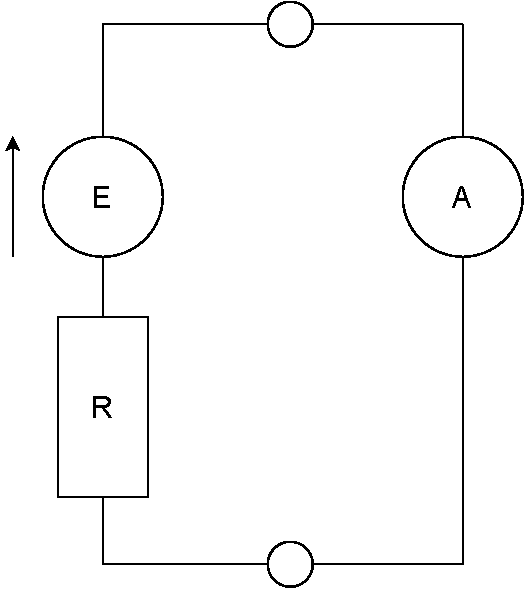
\includegraphics[width=6cm]{schematics/direct.pdf}
	\caption{Direct current measurements schematic}
	\label{fig:direct_schematic}
\end{figure}

\subsubsection{Analog measurements}

The ammeter which we used for analog measurements is was of a 0.5 accuracy class and had $\frac{23}{I_R  [\unit{\milli\ampere}]} + 0.004 [\unit{\ohm}]$ internal resistance (for: $I_R$ -- range).

The measurements along with the results are split into Tables~\ref{tab:direct_analog_1} and~\ref{tab:direct_analog_2}; Tab.~\ref{tab:direct_analog_1} contains the measurement results with only the limiting error applied, whereas Tab.~\ref{tab:direct_analog_2} shows the final results which include the systematic error.

\begin{table}[H]
	\centering
	\begin{tabular}{ c | c | c | c | c | c | c | c }
		$R_C [\unit{\ohm}]$& $\alpha$ & $\alpha_{max}$ & $I_r [\unit{\milli\ampere}]$ & $I [\unit{\milli\ampere}]$ & $\Delta_I [\unit{\milli\ampere}]$ & $\delta_I [\unit{\percent}]$ & $I \pm \Delta_I [\unit{\milli\ampere}]$\\
		\hline
		10  & 66 & 75 & 150.0 & 132.00 & 0.7500 & 0.56819 & $132.0 \pm 0.8$ \\
		30  & 45 & 75 & 75.0 & 45.00 & 0.3750 & 0.83334 & $45.0 \pm 0.4$ \\
		100  & 67 & 75 & 15.0 & 13.40 & 0.0750 & 0.55971 &  $13.40\pm 0.08$\\
		300  & 45.5 & 75 & 7.5 & 4.55 & 0.0375 & 0.82418 & $4.55 \pm 0.04$\\
		1k  & 34 & 75 & 3.0 & 1.36 & 0.0150 & 1.10295 & $1.360\pm 0.016$\\
		3k  & 12 & 75 & 3.0 & 0.48 & 0.0150 & 3.12501 & $0.480\pm 0.016$\\
		10k  & 5 & 75 & 3.0 & 0.20 & 0.0150 & 7.50001 & $0.200\pm 0.016$\\
	\end{tabular}
	\caption{Current measurements for $E\sim\SI{1.3}{\volt}$ (for: $R_C$ -- circuit resistance, $\alpha$ -- actual needle swing, $\alpha_{max}$ -- maximal swing, $I_r$ -- range, $I$ -- measured current, $\Delta_I$ --absolute error, $\delta_I$ -- relative error)}
	\label{tab:direct_analog_1}
\end{table}

\begin{table}[H]
	\centering
	\begin{tabular}{c | c | c | c | c | c | c}
		$R_A [\unit{\ohm}]$ & $\Delta_m I [\unit{\milli\ampere}]$ & $\delta_m I$ & $c [\unit{\milli\ampere}]$ & $I_C [\unit{\milli\ampere}]$ & $I_{exp} [\unit{\milli\ampere}]$ & $I_C \pm \Delta_I [\unit{\milli\ampere}]$\\
		\hline
		0.15734 & -2.07681 & -0.01550 & 2.07681 & 134.07681 &130.00 & $134.1\pm 0.8$\\
		0.31067 & -0.46601 & -0.01025 & 0.46601 & 45.46601 & 43.33 & $45.5\pm 0.4$\\
		1.53734 & -0.20601 & -0.01515 & 0.20601 & 13.60601  & 13.00 & $13.61\pm 0.08$\\
		3.07067 & -0.04658 & -0.01014 & 0.04658 & 4.59658 & 4.33 & $4.60\pm 0.04$\\
		7.67067 & -0.01044 & -0.00762 & 0.01044 & 1.37044 & 1.30 & $1.370\pm 0.016$\\
		7.67067 & -0.00123 & -0.00256 & 0.00123 & 0.48123 & 0.43 & $0.481\pm 0.016$\\
		7.67067 & -0.00016 & -0.00077 & 0.00016 & 0.20016 & 0.13& $0.200\pm 0.016$\\
	\end{tabular}
	\caption{Current measurements for $E\sim\SI{1.3}{\volt}$ (for: $R_A$ -- internal ammeter resistance, $\Delta_m I$ -- systematic error, $\delta_m I$ -- relative error, $c$ -- correction factor, $I_C$ -- calculated current,  $I_{exp}$ -- expected current)}
	\label{tab:direct_analog_2}
\end{table}

Example calculations for $R_C = \SI{300}{\ohm}$ are shown in the equations below.

\begin{equation}
	I = \frac{\alpha\cdot I_r}{\alpha_{max}} = \frac{45.5\cdot \SI{7.5}{\milli\ampere}}{75} = \SI{4.55}{\milli\ampere}
\end{equation}

\begin{equation}
	\Delta_I = \frac{I_r\cdot cl}{100\unit{\percent}} = \frac{\SI{7.5}{\milli\ampere}\cdot 0.5\unit{\percent}}{100\unit{\percent}} = \SI{0.0375}{\milli\ampere}
\end{equation}

\begin{equation}
	\delta_I = \frac{\Delta_I}{I}\cdot 100\unit{\percent} = \frac{\SI{0.0375}{\milli\ampere}}{\SI{4.55}{\milli\ampere}}\cdot 100\unit{\percent} \approx 0.82418\unit{\percent}
\end{equation}

\begin{equation}
	R_A = \frac{23}{I_R  [\unit{\milli\ampere}]} + 0.004 [\unit{\ohm}] = \frac{23}{\SI{7.5}{\milli\ampere}} + \SI{0.004}{\ohm} \approx \SI{3.07067}{\ohm}
\end{equation}

\begin{equation}
	\Delta_m I = -I_A \cdot\frac{R_A}{R_C} = -\SI{4.55}{\milli\ampere}\frac{\SI{3.07067}{\ohm}}{\SI{300}{\ohm}} \approx -\SI{0.04658}{\milli\ampere}
\end{equation}

\begin{equation}
	\delta_m I = -\frac{R_A}{R_A + R_C} = -\frac{\SI{3.07067}{\ohm}}{\SI{3.07067}{\ohm} + \SI{300}{\ohm}} \approx -0.01014
\end{equation}

\begin{equation}
	c = -\Delta_m I = -(-\SI{0.04658}{\milli\ampere}) = \SI{0.04658}{\milli\ampere}
\end{equation}

\begin{equation}
	I_C = I + c = \SI{4.55}{\milli\ampere} +\SI{0.04658}{\milli\ampere} = \SI{4.59658}{\milli\ampere}
\end{equation}

\begin{equation}
	I_{exp} = \frac{V}{R_C} = \frac{\SI{1.3}{\volt}}{\SI{300}{\ohm}} \approx \SI{0.00433}{\ampere} = \SI{4.33}{\milli\ampere}
\end{equation}

\subsubsection{Digital measurements}

Digital measurements were made using a multimeter. Its internal resistance and accuracy are available in the device manual; for our calculations we chose the least precise accuracy value that is guaranteed to work for one year after device calibration.

The measurements along with the results are split into Tables~\ref{tab:direct_digital_1} and~\ref{tab:direct_digital_2}; Tab.~\ref{tab:direct_digital_1} contains the measurement results with only the limiting error applied, whereas Tab.~\ref{tab:direct_digital_2} shows the final results which include the systematic error.

\subsection{Indirect current measurement}